\chapter{引言}

\section{研究背景与意义}
随着互联网、移动设备等科技的发展,数据也以爆炸性的速度在增长。这些日益增长的数据背后隐藏着许多重要的信息,各个领域,例如商业、科学、医疗等,对这些信息的统计分析挖掘有着很高的热情。联机分析处理(OLAP) \cite{chaudhuri1997overview} 是一种多维度的数据分析技术,能进行大规模数据的分析及统计计算,多用于决策支持系统和数据仓库。

%例如企业可分别从用户维度,产品维度以及订单维度来分析对于不同年龄阶层最受欢迎的产品类型,从而推出针对不同年龄阶层的产品销售计划。由于企业数据的快速增长和累积以及企业对分析历史数据、挖掘商业价值的热情逐渐增高,联机分析处理应用在业界变得越来越受欢迎,开发更高效的 OLAP 技术浪潮应运而生。

数据立方(Data Cube) \cite{gray1997data}是由 Jim Gray 等人于 1996 年提出的,它是一种有效支持 OLAP 应用的多维数据计算模型,是 OLAP 领域中的一项关键技术。它提出通过预先计算数据表中各属性间的所有组合对应的 GroupBy 结果并存储起来,以缩短系统的查询响应时间从而提高应用效率。多维度数据的统计分析在各个领域都有广泛的应用,以下是两个例子。

对于一个公司的销售记录,需要统计每周、每月、每个季度等不同时间跨度的销售量,同时还要考虑地区维度、用户维度、商品维度等多个维度不同组合的销售量。销售人员、公司高层等都会根据各自需要查询这些销售统计信息,并且很大部分的销售统计信息会被反复查询,例如每个地区每月的销售量、各个地区每月最畅销的商品等。若每一次的查询都从原始数据表中扫描计算,会耗费非常大的时间与浪费不必要的计算资源。因此可对这些不同维度组合的统计信息提前计算并且存储计算结果,之后的每一次查询都从已计算好的结果中直接读取获得,从而可缩短查询响应时间。

对于一个站点的用户搜索记录,一般包括了不同地区的用户在不同的时间点查询的内容。对不同用户的搜索内容进行统计,有力利于站点的广告投放。通常情况下,用户具有区域性特征,因此将用户维度与地区维度相结合进行统计,可得出更有效的统计信息。同时,由于各地区的时差等原因,用户在不同时间点的搜索频率、活跃度也会有所差异,结合用户维度、时间维度、地区维度统计活跃度可有利于站点合理地分配资源,避免资源的浪费或者分配资源不足的情况。

以上例子的这些统计信息都可转换成GroupBy的计算。并且这些统计信息不仅仅是一个GroupBy计算,而是多个维度多种组合的GroupBy计算,而这些组合之间是有一定联系的,因此可以利用各个GroupBy组合之间的一些共享关系进行计算,从而提高计算效率。这也是数据立方的核心思想所在。

介绍分布式

分布式与数据立方结合

%在现实应用中,数据立方的高效计算是实例化数据立方的关键。 
%随着数据的爆炸性增长,传统的对数据处理计算分析的方法已无法满足当前的需求。仅仅将传统算法与分布式机械地结合,并不能充分利用两者各自的优势。\cite{cuzzocrea2011analytics} \cite{cuzzocrea2013data} \cite{cuzzocrea2013big} 中提出了一些由于数据增长给数据仓库、OLAP 带来的挑战,其中包括大数据的存储与分布、可扩展问题、ETL过程、多维数据的建模、分析、查询等等。
%数据立方是 OLAP 领域内一项关键技术,数据立方的高效计算可大幅度提高 OLAP 对查询的相应时间随着数据的急剧增加,

%如 HBase \cite{hbase},一种基于 Hadoop 的面向列存储的数据库,是一个结构化数据的分布式存储系统。它利用 HDFS 为其提供高可靠的底层存储支持,利用 MapReduce 为其提供高性能的计算能力,能够快速的定位并访问存储于 HDFS 上数十亿行的数据,同时还可利用 Pig \cite{pig} 或 Hive \cite{hive} 为其提供高层语言支持。

%如前雅虎搜索与运计算首席科学家,现微软技术会士 Raghu Ramakrishnan 则带领其团队进行 Data Cube 与 MapReduce 的技术整合,提出了 MR-Cube 方案 \cite{nandi2012data} \cite{nandi2011distributed},针对 MapReduce 框架提出了 Data Cube 的实例化计算方法,并提出了 2 种 整体性度量在分布式计算下的解决方案。MR-Cube 的思想现也在 Pig 开源项目上进行实现 \cite{mrcubepig}。

%随着计算机的普及,计算机逐渐被各行各业用于复杂的数据计算。由于许多项目的数据计算量过大,复杂性过高,

\section{专业术语}

\subsection{数据立方}
数据立方 (Data Cube) \cite{gray1997data} 是一种多维数据计算模型。该模型是针对事实表中各维度的所有组合对应的聚集计算,即各个维度所有组合的 GroupBy 计算。所有 GroupBy 结果构成数据立方。它利用各个组合之间的关系,提高计算效率。在 OLAP 术语中,聚合属性称为维属性, 被计算的属性称为度量属性。

%如图\ref{fact_table_data_cube} 所示,(a) 为事实表 R, A、B、C 为它的维属性,M 为它的度量属性。(b) 为基于事实表 R 构建的数据立方。(b) 中的每个视图代表某个特定维属性组合的 GroupBy 结果。

%\begin{figure}[!htb]
%\centering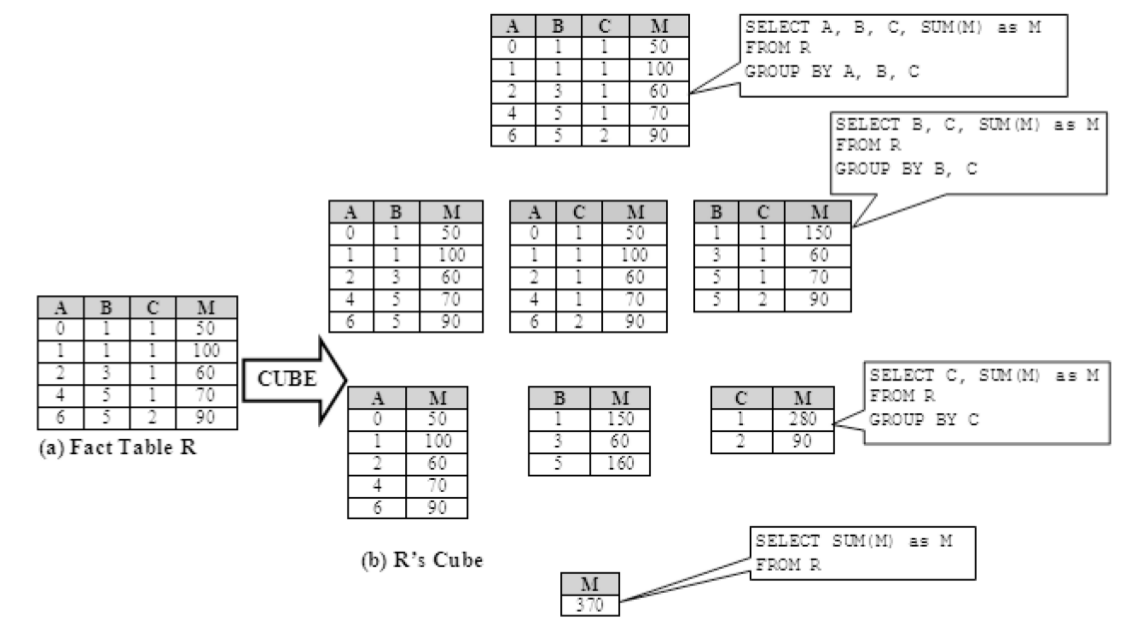
\includegraphics[width=6in]{picture/ch_preliminary/fact_table_data_cube} 
%\caption{事实表与数据立方}\label{fact_table_data_cube} 
%\end{figure} 

\subsection{Lattice, Region, Group}

%对于图\ref{fact_table_data_cube} 中的所有GroupBy,可用另一种方式表示,如图\ref{abc_lattice} 所示,这种结构称为 Lattice。

对于一个事实表中所有的GroupBy可使用一种称为 Lattice 的结构表示,如图\ref{abc_lattice} 所示。

\begin{figure}[!htb]
\centering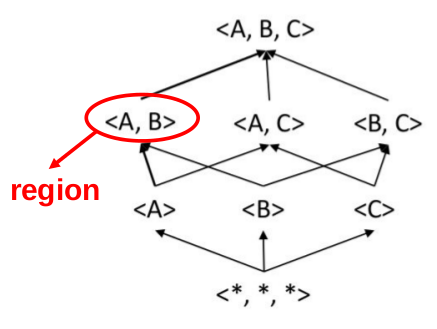
\includegraphics[width=2in]{picture/ch_preliminary/abc_lattice} 
\caption{ABC Lattice}\label{abc_lattice} 
\end{figure} 

在这个lattice中,有维属性组合对应的所有 GroupBy 类型,每个节点表示一种 GroupBy 类型。在lattice中的每个节点称为一个region,也就是一种 GroupBy 类型。
%箭头连接的两个节点表示它们有父子关系。例如Region(AB)与Region(A)之间有箭头连接,Region(AB)为父,Region(A)为子,表示GroupBy(A)的结果可从GroupBy(AB)的结果计算获得。

一个 region 内有多个 group。group 指的是一个
region中带有具体值的 GroupBy。如表\ref{groupby_a_table}是Region(A)(即GroupBy(A))中的group。

\begin{table}[!ht]
\begin{center}
\begin{tabular}{|c|c|}
\hline 
A & M \\ 
\hline 
0 & 50 \\ 
\hline 
1 & 100 \\ 
\hline 
2 & 60 \\ 
\hline 
4 & 70 \\ 
\hline 
6 & 90 \\ 
\hline 
\end{tabular} 
\end{center}
\caption{GroupBy(A)}\label{groupby_a_table}
\end{table}

在表\ref{groupby_a_table}中,Region(A) 中有5个Group,分别是Group(A=0), Group(A=1), Group(A=2), Group(A=4), Group(A=6)。

%从lattice中可见,当一个事实表有 D 个维属性时,它对应的数据立方就会有${2}^{D}$个region,也即有 ${2}^{D}$ 种不同类型的 GroupBy。最简单直接(Naive)的数据立方实现方法,是对每个region进行独立计算并把结果存储起来。对于一张事实表,随着他的维属性数量的增加,它相对应的数据立方的计算与存储代价就会呈指数增长。于是,在 OLAP 中,如何从立方计算、立方存储这两个角度高效地实例化数据立方已成为业界内广泛讨论的一个研究课题。


\subsection{度量}

度量,即对GroupBy的多条数据进行聚合计算,例如SUM,AVG,MEDIAN等。

度量函数一般分为两大类, 分别代数度量(Algebraic)和整体性度量(Holistic)。

以下使用一个二维的数据集$\left\{ {X}_{ij}|i=1,...I; j=1,...J \right\}$分别说明这三种度量函数的区别。

\begin{itemize}

%\item \textbf{分布度量}
%对于分布度量函数 F(),如果存在一个辅助函数 G() 能令 $F(\text\{ {X}_{i,j} \text\}) = G(\text\{ F(\text\{ {X}_{i,j}|i=1,...,I \text\})|j=1,...J \text\})$,则度量函数 F() 为分布度量函数。常见的分布度量函数有 COUNT(), MIN(), MAX(), SUM()。大部分分布度量函数中 $F=G$,但COUNT() 除外。在COUNT()度量函数中,$G=SUM()$。

\item \textbf{代数度量}

对于代数度量函数 F(),如果存在辅助两个函数 G() 和 H(),其中 G() 的输出结果是固定数量的 M 条记录,并且满足$F(\text\{ {X}_{i,j} \text\}) = H(\text\{ G(\text\{ {X}_{i,j}|i=1,...,I \text\})|j=1,...J \text\})$。常见的代数度量函数有AVG(),MaxN(),MinN(),标准差等。例如对于AVG(),函数G()的输出是子集的和以及数量,H()函数则把将各个子集的和相加再除以数量的总和。代数度量的关键是,函数G()的输出结果的数据量是固定的。例如AVG(),无论数据怎么划分,函数G()的输出都是两个值,一个是和,另一个是数量。

\item \textbf{整体性度量}

对于整体性性度量函数 F(),其中间结果,即各个子集的计算结果的数据量大小是不确定的。常见的整体性度量有Median(), Mode(), RANK(), DISTINCT()等。例如使用 DISTINCT()计算一个数列中出现多少不同的数值。若将该数列随意划分,那么每个子数列输出的中间结果仍可能是一个列表,该列表记录了子数列出现哪些数值,即将重复的数值去除。然后再对这些中间结果计算 DISTINCT()。在最坏的情况下,每个子数列输出的中间结果可能就是它本身,因为无重复的数值。

\end{itemize}

%之所以要对度量函数进行分类是因为其会影响数据的划分以及数据立方的计算。论文研究的环境是分布式,因此数据划分是必然的。对于以上三种度量,在分布度量与代数度量下,数据无论如何划分,使用辅助函数都能计算出最终结果,并且中间结果的数据量是确定的。但对于整体性度量,数据无法随意划分,或者数据的随意划分对其计算的意义并不大,因为中间结果数据量的不确定导致中间数据的维护代价可能很大。然而这并不代表数据不能划分。在后面的章节中会提到,对于整体性度量按照一定的方法对数据进行划分,也能令中间结果的数据大小是确定的。为了方便,在之后的阐述中,将分布度量与代数度量都归为代数度量。


\section{当前研究现状}


\cite{agarwal1996computation} \cite{beyer1999bottom} 是较为流行且通用的数据立方计算方法。根据不同角度与特殊场景,业界一直在探讨数据立方计算的优化 \cite{xin2003star} \cite{harinarayan1996implementing} \cite{zhao1997array} \cite{han2001efficient} \cite{wang2002condensed}。\cite{ng2001iceberg} \cite{dehne2002parallelizing} 还提出了在小集群上的并行数据立方计算的方法。但随着数据量的急剧增长,单机和小集群上数据立方的计算方法已无法满足数据立方的计算要求。


面对惊人的计算量,选择大量廉价的计算机组成一个分布式计算系统,是一个能够在满足时间和成本代价的基础上解决计算难题的办法。谷歌提出了 MapReduce \cite{dean2008mapreduce}分布式计算框架。随着 Hadoop \cite{hadoop}开源项目的发展,MapReduce 已成为目前业界流行的分布式计算框架,它具有高度的集群稳定性及高效的规模扩展性。它不仅在处理非结构化数据上有卓越的表现,业界还不断扩展它处理结构化数据的能力 \cite{hbase} \cite{abouzeid2009hadoopdb} \cite{buck2011scihadoop} \cite{pig} \cite{hive}。因此探索如何在分布式计算框架MapReduce下高效地完成数据立方的计算成为势在必行的一个趋势
 \cite{abello2011building} \cite{wang2010mapreducemerge} \cite{sergey2009applying} \cite{lee2012efficient} \cite{wang2013scalable}。
 
 Raghu Ramakrishnan 团队提出的 MapReduce DataCube 方案 \cite{nandi2012data} \cite{nandi2011distributed}(以下简称MR-Cube),是当前 MapReduce 与数据立方的最佳结合。MR-Cube解决了整体性度量函数与MapReduce的结合、数据划分、中间数据过多、合并计算等问题。虽然它实现了数据立方与 MapReduce 的高效结合,但其仍存在缺陷,尤其是在一些倾斜的数据集下,该算法的数据划分方法分会产生不必要的划分。并且MR-Cube使用取模的方法划分数据,在一些情况下会导致不均匀的划分。同时它对合并计算只给出了一些建议遵循的规则,并没有给出具体的简单有效的合并方法。此外,MR-Cube 使用了 BUC \cite{beyer1999bottom} 的算法计算 MapReduce 下的数据立方,然而数据立方的实现技术除了 BUC 外,还有 PipeSort,PipeHash \cite{agarwal1996computation} 等。这些方法与 BUC 相比,更能利用 MapReduce 框架的特性。因此可使用其他数据立方计算方法取代 BUC,从而使数据立方计算与MapReduce有更好的整合。

\section{论文主要工作及贡献}

本文探讨当前数据立方计算的研究现状,主要针对Raghu Ramakrishnan 团队提出的 MR-Cube 方案 \cite{nandi2012data} \cite{nandi2011distributed},分析其优缺点。根据MR-Cube的不足以及可改进的地方,借鉴\cite{tao2013minimal} 中将TeraSort 与 GroupBy 结合的方法 以及 将 MapReduce 与 PipeSort 结合,提出了TSP-Cube 计算方法。TSP-Cube 使用 Tera Sort 的思想提出更具有通用性的对倾斜数据的划分方法;并且使用 PipeSort 替代 BUC 方法实现基于 MapReduce 的数据立方,从而更充分利用MapReduce框架的特性。同时,针对层次型的数据集以及结合PipeSort的特征,提出简单且有效的Pipeline生成方案。最后通过实验比较TSP-Cube与多种数据立方计算方法在性能、负载等方面的优势,并且根据实验结果总结出两种不同类型的度量函数适用的数据立方计算方法。

%从而为后续的MapReduce 与数据立方计算的优化实现提供研究经验支持。

\section{论文结构安排}
本文内容安排如下,第2章介绍与数据立方相关的基础知识,第3章探讨当前数据立方计算的研究现状,第4章具体分析MR-Cube的贡献以及不足,第5章提出TSP-Cube方法,并对其进行详细的理论分析,第6章阐述实验结果与结果分析,第7章为总结与展望。

